\documentclass[table]{beamer}
\usepackage{amsmath, amsthm}
\usepackage{tabularx}
\usepackage{multirow}
\usepackage{tikz}
\usepackage{verbatim}
\usepackage{graphicx}
\usepackage{xcolor}
\usepackage{}
\usetikzlibrary{positioning}
% for gadget figure
\usetikzlibrary{automata, shadows, calc, fit}

\definecolor{felix_bg}{HTML}{f3eede}
\definecolor{felix_text}{HTML}{308f94}


% Problem style
\usepackage{xspace}
\newcommand{\probname}[1]{\textnormal{\textsc{#1}}\xspace}
\newcommand{\gm}[0]{\probname{Gerrymandering}}
\newcommand{\lp}[0]{\probname{$k$-Labeled Path}}
\newcommand{\scov}[0]{\probname{Set Cover}}
\newcommand{\wgm}[0]{\probname{Weighted Gerrymandering}}

\DeclareMathOperator*{\argmax} {arg\ max}

% observation
\newtheorem{observation}{Observation}

% Macros
\newcommand{\n}{n} % Set Cover n
\newcommand{\m}{m} % Set Cover m
\newcommand{\D}{\mathcal{D}}
\newcommand{\Un}{\mathcal{U}}
\newcommand{\F}{\mathcal{F}}

% problem box
\newcommand{\problembox} [3] {
    \noindent
    \vspace{\dimexpr\parskip+1.35ex}
    \begin{tikzpicture}
        \node[draw=black!40, rounded corners, inner sep=2ex] (content) {
            \begin{tabularx} {\dimexpr\columnwidth-4ex} {l X}
                \textbf{Input:} & #2\\
                \textbf{Problem:} & #3\\
            \end{tabularx}
        };
        
        \node[inner sep=3pt, fill=white, anchor=north west] at ($(content.north west) + (2ex, 1.35ex)$) {\probname{#1}};
    \end{tikzpicture}
    \ignorespaces
}

% colors
\definecolor{orange}{RGB}{230,159,0}
\definecolor{skyblue}{RGB}{86,180,233}
\definecolor{bluegreen}{RGB}{0,158,115}
\definecolor{yellow}{RGB}{240,228,66}
\definecolor{blue}{RGB}{0,114,178}
\definecolor{vermillion}{RGB}{213,94,0}
\definecolor{redpurple}{RGB}{204,121,167}

\addtobeamertemplate{navigation symbols}{}{%
    \usebeamerfont{footline}%
    \usebeamercolor[fg]{footline}%
    \hspace{1em}%
    \insertframenumber/13
}

\title{Gerrymandering Trees: Parameterized Hardness}
\author{\textcolor{red}{Andrew Fraser}, Brian Lavallee, Blair D. Sullivan}
\date{Symposium on Algorithmic Game Theory, September 2023}


\begin{document}

	\begin{frame}
		\titlepage
	\end{frame}

	%{\setbeamercolor{background canvas}{bg=felix_bg}

\begin{frame}[t]
	\frametitle{Defining Gerrymandering}
	\small
	\problembox{Gerrymandering}
	{A graph $G = (V,E)$, a set of candidates $C$, a candidate function $\chi: V \rightarrow C$, a weight function $w: V \rightarrow \mathbb{N}$, a preferred candidate $p \in C$, and an integer $k \in \mathbb{N}$.}
	{Is there a district-partition of $V$ into $k$ districts such that $p$ wins more districts than any other candidate?}

	\begin{figure}
		\begin{center}
			
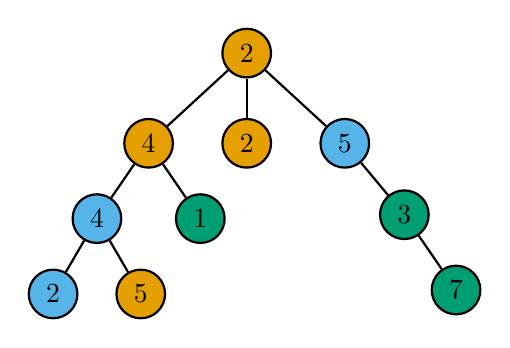
\begin{tikzpicture}
	\tikzstyle{node} = [circle, draw, thick]
	\tikzstyle{edge} = [thick]

	\node (1) [node, fill=orange] {4};
	\node (2) [node, fill=orange, right=0.6cm of 1] {2};
	\node (3) [node, fill=skyblue, right=0.6cm of 2] {5};
	\node (4) [node, fill=orange, above=0.5cm of 2] {2};

	\node (5) [node, fill=bluegreen, below right=0.45cm and 0.3cm of 3] {3};
	\node (6) [node, fill=bluegreen, below right=0.5cm and 0.2cm of 1] {1};
	\node (12) [node, fill=bluegreen, below right=0.5cm and 0.2cm of 5] {7};

	\node (9) [node, fill=skyblue, below left=0.5cm and 0.2cm of 1] {4};
	\node (10) [node, fill=skyblue, below left=0.5cm and 0.1cm of 9] {2};
	\node (11) [node, fill=orange, below right=0.5cm and 0.1cm of 9] {5};

	\draw (1) edge [edge] (4);
	\draw (1) edge [edge] (6);
	\draw (1) edge [edge] (9);
	\draw (2) edge [edge] (4);
	\draw (3) edge [edge] (5);
	\draw (3) edge [edge] (4);

	\draw (9) edge [edge] (10);
	\draw (11) edge [edge] (9);
	\draw (12) edge [edge] (5);

	\tikzstyle{node} = []
\end{tikzpicture}

		\end{center}
	\end{figure}
\end{frame}

\begin{frame}[t]
	\frametitle{Gerrymandering Example}
	\begin{figure}
		\begin{center}
			
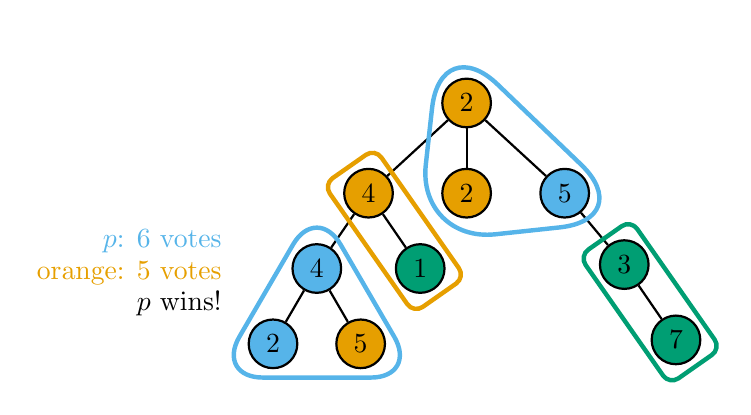
\begin{tikzpicture}
	\tikzstyle{node} = [circle, draw, thick]
	\tikzstyle{edge} = [thick]

	\node (1) [node, fill=orange] {4};
	\node (2) [node, fill=orange, right=0.6cm of 1] {2};
	\node (3) [node, fill=skyblue, right=0.6cm of 2] {5};
	\node (4) [node, fill=orange, above=0.5cm of 2] {2};

	\node (5) [node, fill=bluegreen, below right=0.45cm and 0.3cm of 3] {3};
	\node (6) [node, fill=bluegreen, below right=0.5cm and 0.2cm of 1] {1};
	\node (12) [node, fill=bluegreen, below right=0.5cm and 0.2cm of 5] {7};

	\node (9) [node, fill=skyblue, below left=0.5cm and 0.2cm of 1] {4};
	\node (10) [node, fill=skyblue, below left=0.5cm and 0.1cm of 9] {2};
	\node (11) [node, fill=orange, below right=0.5cm and 0.1cm of 9] {5};

	\draw (1) edge [edge] (4);
	\draw (1) edge [edge] (6);
	\draw (1) edge [edge] (9);
	\draw (2) edge [edge] (4);
	\draw (3) edge [edge] (5);
	\draw (3) edge [edge] (4);

	\draw (9) edge [edge] (10);
	\draw (11) edge [edge] (9);
	\draw (12) edge [edge] (5);

	\tikzstyle{node} = []

	\onslide<2-3> {
		\node (phint) [node, text=skyblue, above left=0.8cm and 0.3cm of 10] {$p$: 6 votes};
		\node (ohint) [node, text=orange, above left=0.4cm and 0.3cm of 10] {orange: 5 votes};
		\node (distresult) [node, above left=0cm and 0.3cm of 10] {$p$ wins!};
		\draw[ultra thick, rounded corners=6mm, color=skyblue] ($(9.north)+(0,0.5)$) -- ($(10.south west)+(-0.5,-0.2)$) -- ($(11.south east)+(0.5,-0.2)$) -- cycle;
	}

	\onslide<3> {
		\draw[ultra thick, rotate=-55, rounded corners, color=orange] ($(1.north west)+(-0.1,0.45)$) rectangle ($(6.south east)+(0.1, -0.45)$);

		\draw[ultra thick, rounded corners=10mm, color=skyblue] ($(4.north west)+(-0.1,0.7)$) -- ($(2.south west)+(-0.4,-0.4)$) -- ($(3.south east)+(0.7,-0.1)$) -- cycle;

		\draw[ultra thick, rotate=-55, rounded corners, color=bluegreen] ($(5.north west)+(-0.1, 0.45)$) rectangle ($(12.south east)+(0.1, -0.45)$);
	}
	
	

\end{tikzpicture}

		\end{center}
	\end{figure}

	\begin{itemize}
		\item Candidates $\rightarrow$ color. Our preferred candidate $p$ is blue.
		\item Weights $\rightarrow$ votes.
		\onslide<3> {
			\item Our candidate $p$ wins twice, others win once. Therefore, this is a YES-instance.
			\item This instance has $k=4$ districts.
		}
	\end{itemize}
\end{frame}

\begin{frame}[t]
	\frametitle{Parameterized Complexity}
	What if our problem considers an additional parameter $k$ such that $n >> k$?
	\vspace{1.0cm}
	\begin{itemize}
		\item FPT: There exists an algorithm that runs in $O(f(k)n^{O(1)})$ time.
		\vspace{1.0cm}
		\item W[2]-Hard: No FPT algorithm exists assuming $FPT \neq XP$.
	\end{itemize}
\end{frame}
	\begin{frame}[t]
    \frametitle{Known Results}

    \begin{itemize}
		\item
		Parameter: $k$
	\end{itemize}

	\vspace{0.5em}
    
\renewcommand{\arraystretch}{1.3}
\newcolumntype{Y}{>{\centering\arraybackslash}X}
\begin{tabularx}{\textwidth}{|c||c|Y|Y|Y|}
	\hline

	&
	$K_{2,n}$/General &
	Trees &
	Paths &
	Stars \\

	\hline
	\hline

	XP &
	\cellcolor{gray} Ito 3.1 &
	\cellcolor{blue} Ito 4.1 &
	\cellcolor{blue} &
	\cellcolor{blue} \\

	\hline

	FPT &
	\cellcolor{gray} &
	\only<4>{\cellcolor{red}???} &
	\cellcolor{blue} Gupta 1.2 &
	\cellcolor{blue} \\

	\hline

	Poly &
	\cellcolor{gray} &
	\cellcolor{gray} Ito 3.3 &
	\cellcolor{gray} Bentert 1 &
	\cellcolor{blue} Ito 4.2 \\

	\hline
\end{tabularx}
\renewcommand{\arraystretch}{1}

        \only<2-3> {
        \begin{itemize}
            \item $K_{2,n}$ for $n=5$: \only<3> {One vertex deletion from a star!}
        \end{itemize}
        \begin{center}
        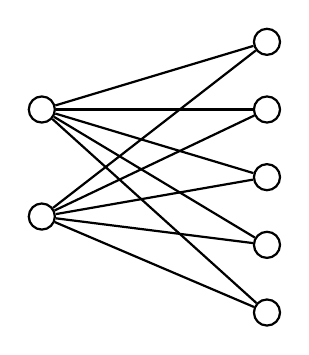
\begin{tikzpicture}
    \tikzstyle{node} = [circle, draw, thick, minimum size = 1.3pt]
	\tikzstyle{edge} = [thick]

    \node (a1) [node] {};
    \node (b2) [node, right=2.5cm of a1] {};
    \node (b3) [node, below=0.5cm of b2] {};
    \node (b1) [node, above=0.5cm of b2] {};
    \node (b4) [node, below=0.5cm of b3] {};
    \node (b5) [node, below=0.5cm of b4] {};

    \draw (a1) edge [edge] (b1);
    \draw (a1) edge [edge] (b2);
    \draw (a1) edge [edge] (b3);
    \draw (a1) edge [edge] (b4);
    \draw (a1) edge [edge] (b5);

    \onslide<2> {
        \node (a2) [node, below=1.0cm of a1] {};
        \draw (a2) edge [edge] (b1);
        \draw (a2) edge [edge] (b2);
        \draw (a2) edge [edge] (b3);
        \draw (a2) edge [edge] (b4);
        \draw (a2) edge [edge] (b5);
    }

\end{tikzpicture}
        \end{center}
    }
    \onslide<4> {
    \vspace{0.5em}
    Our results on trees parameterized by $k$ districts:
    \begin{itemize}
        \color{red}
        \item W[2]-Hard with depth=2
        \item W[2]-Hard with $\ell$ leaves
        \item An $O(n^{\ell}f(k))$ algorithm (XP in $\ell$, FPT in $k$)
    \end{itemize}
    }
\end{frame}

\begin{frame}[t]
    \frametitle{Reducing from...}
    \problembox{Set Cover}
    {A set of elements $\Un = \{e_1, \dots, e_n\}$, a family of sets $\F = \{S_1, \dots, S_m\}$, and an integer $t \in \mathbb{N}$.}
    {Is there a subset $X \subseteq \F$ such that $|X| \leq t$ and $\bigcup_{S \in X} S = \Un$?}

    \begin{figure}
        \begin{flushleft}
		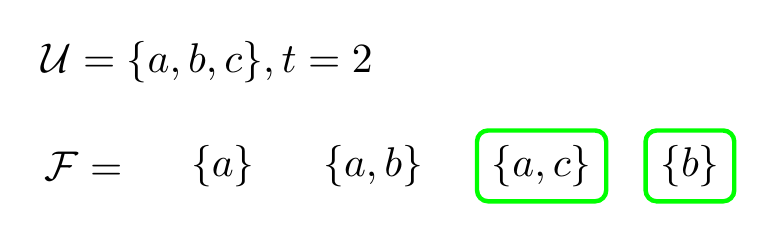
\begin{tikzpicture}
    \tikzstyle{node} = [scale=1.5];

    \onslide<2-5> {

    \node (U) [node] {$ \Un = \{a, b, c\}, t=2$};

    \node (F) [node, below left=0.5cm and -1.4cm of U] {$\F = $};
    \node (s1) [node, right=0.5cm of F] {$\{a\}$};
    \node (s2) [node, right=0.5cm of s1] {$\{a, b\}$};
    \node (s3) [node, right=0.5cm of s2] {$\{a, c\}$};
    \node (s4) [node, right=0.5cm of s3] {$\{b\}$};
    }
    \onslide<3-5>{
        \draw[ultra thick, rounded corners, color=green] ($(s3.north west)$) rectangle ($(s3.south east)$);
        \draw[ultra thick, rounded corners, color=green] ($(s4.north west)$) rectangle ($(s4.south east)$);
    }

\end{tikzpicture}
        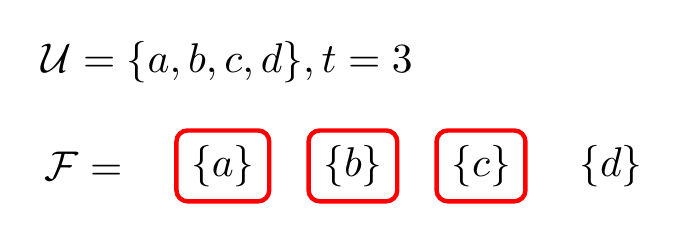
\begin{tikzpicture}
    \tikzstyle{node} = [scale=1.5];

    \onslide<4-5> {

    \node (U) [node] {$ \Un = \{a, b, c, d\}, t=3$};

    \node (F) [node, below left=0.5cm and -1.4cm of U] {$\F = $};
    \node (s1) [node, right=0.5cm of F] {$\{a\}$};
    \node (s2) [node, right=0.5cm of s1] {$\{b\}$};
    \node (s3) [node, right=0.5cm of s2] {$\{c\}$};
    \node (s4) [node, right=0.5cm of s3] {$\{d\}$};
    }
    
    \onslide<5>{
        \draw[ultra thick, rounded corners, color=red] ($(s1.north west)$) rectangle ($(s1.south east)$);
        \draw[ultra thick, rounded corners, color=red] ($(s2.north west)$) rectangle ($(s2.south east)$);
        \draw[ultra thick, rounded corners, color=red] ($(s3.north west)$) rectangle ($(s3.south east)$);
    }

\end{tikzpicture}
        \end{flushleft}
	\end{figure}
\end{frame}

\begin{frame}[t]
    \frametitle{Reducing From Set Cover to Gerrymandering}
    \scov is W[2]-Hard with respect to $t$, size of our cover.

    We want to show that \gm is W[2]-Hard with respect to $k$ districts + $\ell$ leaves.

    \vspace{1.0cm}
    To do this, we must solve \scov using \gm.
    \begin{itemize}
        \item Our preferred candidate wins $\leftrightarrow$ we have a set cover
    \end{itemize}
    
    \vspace{1.0cm}
    Additionally, $k$ and $\ell$ must be bounded by some function of $t$.
\end{frame}

\begin{frame}[t]
    \frametitle{W[2]-Hardness In Trees with $\ell$ Leaves}

    \begin{figure}
		\begin{center}
			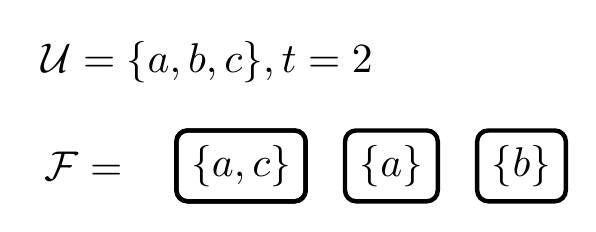
\begin{tikzpicture}
    \tikzstyle{node} = [scale=1.5];

    \node (U) [node] {$ \Un = \{a, b, c\}, t=2$};

    \node (F) [node, below left=0.5cm and -1.4cm of U] {$\F = $};
    \node (s1) [node, right=0.5cm of F] {$\{a, c\}$};
    \node (s2) [node, right=0.5cm of s1] {$\{a\}$};
    \node (s3) [node, right=0.5cm of s2] {$\{b\}$};

    \onslide<6-8> {
        \draw[ultra thick, rounded corners, color=black] ($(s1.north west)$) rectangle ($(s1.south east)$);
    }

    \onslide<9-14> {
        \draw[ultra thick, rounded corners, color=black] ($(s2.north west)$) rectangle ($(s2.south east)$);
    }

    \onslide<17-18> {
        \draw[ultra thick, rounded corners, color=black] ($(s1.north west)$) rectangle ($(s1.south east)$);
        \draw[ultra thick, rounded corners, color=black] ($(s3.north west)$) rectangle ($(s3.south east)$);

    }
    
    %\draw[ultra thick, rounded corners, color=green] ($(s1.north west)$) rectangle ($(s1.south east)$);
    %\draw[ultra thick, rounded corners, color=green] ($(s3.north west)$) rectangle ($(s3.south east)$);

\end{tikzpicture}
		\end{center}
	\end{figure}

    \begin{figure}
		\begin{center}
			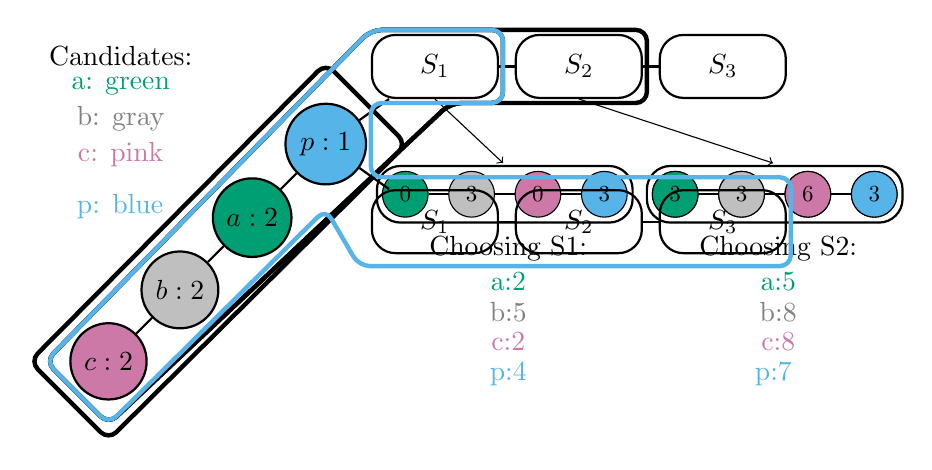
\begin{tikzpicture}
    \tikzstyle{node} = [circle, draw, thick, minimum size=0.7cm]
	\tikzstyle{edge} = [thick]
    \tikzstyle{gnode} = [rectangle, draw, thick, minimum width=1.6cm, minimum height=0.8cm, rounded corners=0.3cm]
    \tikzstyle{znode} = [circle, draw, minimum size=0.7cm, scale=0.83]

    \onslide<2-18> {
        \node (r) [node, fill=skyblue] {$p:1$};
        \node (plabel) [text=skyblue, above left= -1.45cm and 1.57cm of r] {p: blue};
        \node (candlabel) [text=black, above left= 0.5cm and 1.2cm of r] {Candidates:};
    }

    \onslide<3-18> {
    %\node (g11) [gnode, below right=0.2cm and 0.2cm of r] {$S_1$};
    %\node (gi1) [gnode, right=0.2cm of g11] {$S_2$};
    %\node (gn1) [gnode, right=0.2cm of gi1] {$S_3$};
    \node (g12) [gnode, above right=0.2cm and 0.2cm of r] {$S_1$};
    \node (gi2) [gnode, right=0.2cm of g12] {$S_2$};
    \node (gn2) [gnode, right=0.2cm of gi2] {$S_3$};
    %\draw (r) edge [edge] (g11);
    %\draw (g11) edge [edge] (gi1);
    %\draw (gi1) edge [edge] (gn1);
    \draw (r) edge [edge] (g12);
    \draw (g12) edge [edge] (gi2);
    \draw (gi2) edge [edge] (gn2);
    
    }

    %\node (e1) [znode, fill=vermillion, below right=0.75cm and -0.56cm of g11] {$v_i^1$};
    %\node (e2) [minimum size = 0.5cm, right=0.25cm of e1] {$\dots$};
    %\node (en) [znode, fill=redpurple, right=0.25cm of e2] {$v_i^n$};
    %\node (x) [znode, fill=bluegreen, right=0.25cm of en] {$x_i$};

    \onslide<4-18> {
        \node (e1) [node, fill=bluegreen, below left=0.2cm and 0.2cm of r] {$a:2$};
        \node (e2) [node, fill=lightgray, below left = 0.2cm and 0.2cm of e1] {$b:2$};
        \node (en) [node, fill=redpurple, below left=0.2cm and 0.2cm of e2] {$c:2$};
        \draw (r) edge [edge] (e1);
        \draw (e1) edge [edge] (e2);
        \draw (e2) edge [edge] (en);

        \node (alabel) [text=bluegreen, below=-0.1cm of candlabel] {a: green};
        \node (blabel) [text=gray, below=-0.1cm of alabel] {b: gray};
        \node (clabel) [text=redpurple, below=-0.1cm of blabel] {c: pink};
    }

    \onslide<5> {
        \draw[ultra thick, rounded corners, color=black] ($(r.north) + (0, 0.5)$) -- ($(r.east) + (0.5, 0)$) -- ($(en.south) + (0, -0.5)$) -- ($(en.west) + (-0.5, 0)$) -- cycle;
        %\draw[ultra thick, rounded corners, color=black] ($(g12.north west) + (0, 0.05)$) -- ($(g12.north east) + (0.05, 0.05)$) -- ($(g12.south east) + (0.05, -0.05)$) -- ($(g12.south) + (0.2, -0.05)$) -- ($(en.south) + (0.0, -0.3)$) -- ($(en.west) + (-0.3, 0.0)$) -- cycle; 
        %\draw[ultra thick, rounded corners, color=skyblue] ($(g12.north west) + (0, 0.05)$) -- ($(g12.north east) + (0.05, 0.05)$) -- ($(g12.south east) + (0.05, -0.05)$) -- ($(g12.south west) + (0, -0.05)$) -- ($(g11.north west) + (0, 0.15)$) -- ($(gn1.north east) + (0.05, 0.15)$) -- ($(gn1.south east) + (0.05, -0.15)$) -- ($(g11.south west) + (-0.15, -0.15)$) -- ($(r.west) + (-0.15, 0.0)$) -- cycle;
        %\draw[ultra thick, rounded corners, color=skyblue] ($(g12.north west) + (0, 0.05)$) -- ($(g12.north east) + (0.05, 0.05)$) -- ($(g12.south east) + (0.05, -0.05)$) -- ($(g12.south west) + (0, -0.05)$) -- ($(g11.north west) + (0, 0.15)$) -- ($(gn1.north east) + (0.05, 0.15)$) -- ($(gn1.south east) + (0.05, -0.15)$) -- ($(g11.south west) + (-0.15, -0.15)$) -- ($(r.south) + (0.0, -0.2)$) -- ($(en.south) + (0.0, -0.3)$) -- ($(en.west) + (-0.3, 0.0)$) -- cycle;
        %\draw[ultra thick, rounded corners, color=skyblue] ($(g12.north west) + (-0.15, 0.15)$) -- ($(g12.north east) + (0.05, 0.15)$) -- ($(g12.south east) + (0.05, -0.15)$) -- ($(g12.south west) + (0, -0.15)$) -- ($(g11.north west) + (0, 0.15)$) -- ($(gn1.north east) + (0.05, 0.15)$) -- ($(gn1.south east) + (0.05, -0.15)$) -- ($(g11.south west) + (-0.15, -0.15)$) -- ($(r.west) + (-0.15, 0.0)$)  -- ($(g12.north west) + (-0.15, 0.15)$);
    }

    \onslide<6-8> {
        \draw[ultra thick, rounded corners, color=black] ($(g12.north west) + (0, 0.05)$) -- ($(g12.north east) + (0.05, 0.05)$) -- ($(g12.south east) + (0.05, -0.05)$) -- ($(g12.south) + (0.2, -0.05)$) -- ($(en.south) + (0.0, -0.3)$) -- ($(en.west) + (-0.3, 0.0)$) -- cycle; 
        %\draw[ultra thick, rounded corners, color=skyblue] ($(g12.north west) + (0, 0.05)$) -- ($(g12.north east) + (0.05, 0.05)$) -- ($(g12.south east) + (0.05, -0.05)$) -- ($(g12.south west) + (0, -0.05)$) -- ($(g11.north west) + (0, 0.15)$) -- ($(gn1.north east) + (0.05, 0.15)$) -- ($(gn1.south east) + (0.05, -0.15)$) -- ($(g11.south west) + (-0.15, -0.15)$) -- ($(r.west) + (-0.15, 0.0)$) -- cycle;
    }

    \onslide<7-14> {
        \node (a1) [znode, fill=bluegreen, below right=1.0cm and -1.4cm of g12] {$0$};
        \node (b1) [znode, fill=lightgray, right=0.25cm of a1] {$3$};
        \node (c1) [znode, fill=redpurple, right=0.25cm of b1] {$0$};
        \node (p1) [znode, fill=skyblue, right=0.25cm of c1] {$3$};

        \draw (a1) edge [edge] (b1);
        \draw (b1) edge [edge] (c1);
        \draw (c1) edge [edge] (p1);

        \draw[thick, rounded corners=0.3cm, color=black] ($(a1.north west) + (-0.15, 0.15)$) rectangle ($(p1.south east) + (0.15, -0.15)$);
        \draw[->] ($(g12.south) + (0, 0)$) -> ($(b1.north) + (0.4, 0.1)$);
    }

    \onslide<8-14> {
        \node (chooses1) [text=black, below right = 0.2cm and -0.87cm of b1] {Choosing S1:};
        \node (atal) [text=bluegreen, below=-0.1cm of chooses1] {a:2};
        \node (btal) [text=gray, below=-0.1cm of atal] {b:5};
        \node (ctal) [text=redpurple, below=-0.1cm of btal] {c:2};
        \node (ptal) [text=skyblue, below=-0.1cm of ctal] {p:4};
    }

    \onslide<9-14> {
        \draw[ultra thick, rounded corners, color=black] ($(g12.north west) + (0, 0.05)$) -- ($(gi2.north east) + (0.05, 0.05)$) -- ($(gi2.south east) + (0.05, -0.05)$) -- ($(g12.south) + (0.2, -0.05)$) -- ($(en.south) + (0.0, -0.3)$) -- ($(en.west) + (-0.3, 0.0)$) -- cycle; 
    }

    \onslide<10-11> {
        \node (a2) [znode, fill=bluegreen, below right=1.0cm and 0.2cm of gi2] {};
    }

    \onslide<10-12> {
        \node (b2) [znode, fill=lightgray, right=0.25cm of a2] {};
    }

    \onslide<10-13> {
        \node (c2) [znode, fill=redpurple, right=0.25cm of b2] {};
    }

    \onslide<10> {
        \node (p2) [znode, fill=skyblue, right=0.25cm of c2] {};
    }

    \onslide<10-14> {
        \draw (a2) edge [edge] (b2);
        \draw (b2) edge [edge] (c2);
        \draw (c2) edge [edge] (p2);

        \draw[thick, rounded corners=0.3cm, color=black] ($(a2.north west) + (-0.15, 0.15)$) rectangle ($(p2.south east) + (0.15, -0.15)$);
        \draw[->] ($(gi2.south) + (0, 0)$) -> ($(b2.north) + (0.4, 0.1)$);

        \node (chooses2) [text=black, below right = 0.2cm and -0.87cm of b2] {Choosing S2:};
    }

    \onslide<11-14> {
        \node (p2) [znode, fill=skyblue, right=0.25cm of c2] {3};
        \node (ptal2) [text=skyblue, right=2.65cm of ptal] {p:7};
    }

    \onslide<12-14> {
        \node (a2) [znode, fill=bluegreen, below right=1.0cm and 0.2cm of gi2] {3};
        \node (atal2) [text=bluegreen, below=-0.1cm of chooses2] {a:5};
    }

    \onslide<13-14> {
        \node (b2) [znode, fill=lightgray, right=0.25cm of a2] {3};
        \node (btal2) [text=gray, below=-0.1cm of atal2] {b:8};
    }

    \onslide<14> {
        \node (c2) [znode, fill=redpurple, right=0.25cm of b2] {6};
        \node (ctal2) [text=redpurple, below=-0.1cm of btal2] {c:8};
    }

    \onslide<16-18> {
        \node (g11) [gnode, below right=0.2cm and 0.2cm of r] {$S_1$};
        \node (gi1) [gnode, right=0.2cm of g11] {$S_2$};
        \node (gn1) [gnode, right=0.2cm of gi1] {$S_3$};

        \draw (r) edge [edge] (g11);
        \draw (g11) edge [edge] (gi1);
        \draw (gi1) edge [edge] (gn1);
    }

    \onslide<18> {
        \draw[ultra thick, rounded corners, color=skyblue] ($(g12.north west) + (0, 0.05)$) -- ($(g12.north east) + (0.05, 0.05)$) -- ($(g12.south east) + (0.05, -0.05)$) -- ($(g12.south west) + (0, -0.05)$) -- ($(g11.north west) + (0, 0.15)$) -- ($(gn1.north east) + (0.05, 0.15)$) -- ($(gn1.south east) + (0.05, -0.15)$) -- ($(g11.south west) + (-0.15, -0.15)$) -- ($(r.south) + (0.0, -0.3)$) -- ($(en.south) + (0.0, -0.3)$) -- ($(en.west) + (-0.3, 0.0)$) -- cycle;
    }

    %\onslide<5-10> {
        %\node (f1) [node, fill=orange, right=0.3cm of gn1] {$f$};
        %\node (fp1) [node, fill=bluegreen, right=0.3cm of f1] {$f'$};

    
        %\node (f2) [node, fill=orange, right=0.3cm of gn2] {$f$};
        %\node (fp2) [node, fill=yellow, right=0.3cm of f2] {$f'$};

        %\draw (gn1) edge [edge] (f1);
        %\draw (f1) edge [edge] (fp1);

    
        %\draw (gn2) edge [edge] (f2);
        %\draw (f2) edge [edge] (fp2);
    %}

    %\onslide<8-10> {
        %\draw[ultra thick, rounded corners, color=bluegreen] ($(f1.north west) + (-0.2, 0.2)$) rectangle ($(fp1.south east) + (0.2, -0.2)$);

        %\draw[ultra thick, rounded corners, color=yellow] ($(gi2.north west) + (-0.05, 0.2)$) rectangle ($(fp2.south east) + (0.2, -0.275)$);
    %}
    %\onslide<3-10> {
        %\node (e1) [node, fill=vermillion, below left=0.2cm and 0.2cm of r] {$a$};
        %\node (e2) [node, fill=lightgray, below left = 0.2cm and 0.2cm of e1] {$b$};
        %\node (en) [node, fill=redpurple, below left=0.2cm and 0.2cm of e2] {$c$};

        %\draw (r) edge [edge] (e1);
        %\draw (e1) edge [edge] (e2);
        %\draw (e2) edge [edge] (en);
    %}

    %\onslide<9-10> {
        %\node (u1) [node, fill=skyblue, above left=0.2cm and 0.2cm of r] {$c_1$};
        %\node (u2) [node, fill=orange, above left=0.2cm and 0.2cm of u1] {$c_2$};
        %\draw (r) edge [edge] (u1);
        %\draw (u1) edge [edge] (u2);
    %}

    %\onslide<10> {
        %\draw[ultra thick, rounded corners, color=skyblue] ($(u1.north west) + (-0.2, 0.2)$) rectangle ($(u1.south east) + (0.2, -0.2)$);
        %\draw[ultra thick, rounded corners, color=orange] ($(u2.north west) + (-0.2, 0.2)$) rectangle ($(u2.south east) + (0.2, -0.2)$);
    %}

    

    %\draw (e1) edge [edge] (e2);
    %\draw (e2) edge [edge] (en);
    %\draw (en) edge [edge] (x);
    %\draw (x) edge [edge] (y);
    %\draw (y) edge [edge] (z);

    %\draw ($(gi1.south west) + (0.1, 0.1)$) -- ($(e1.north) + (-0.27, 0.15)$);
    %\draw ($(gi1.south east) + (-0.1, 0.1)$) -- ($(z.north) + (0.27, 0.15)$);
    %\draw[thick, rounded corners=0.3cm] ($(e1.north west) + (-0.25, 0.25)$) rectangle ($(z.south east) + (0.25, -0.25)$);
\end{tikzpicture}

		\end{center}
	\end{figure}
\end{frame}

\begin{frame}
    \frametitle{W[2]-Hardness In Trees with $\ell$ Leaves}
    \begin{itemize}
        \item Our candidate $p$ wins the root district $\leftrightarrow$ the root district resembles a set cover.
        %\item Create $t$ branches. For each branch, choosing a district $\rightarrow$ choosing a set.
        %\item Put $c_1$ and $c_2$ into their own districts.
        \onslide<2-9> {
            \item Same example: $|\Un| = 3, |\F| = 3$, $t = 2$ sets to choose.
        }
        \onslide<9> {
            \item Note: $k=t+2$ and $\ell = t+2$. Our parameter translates.
        }
    \end{itemize}

    \begin{figure}
		\begin{center}
			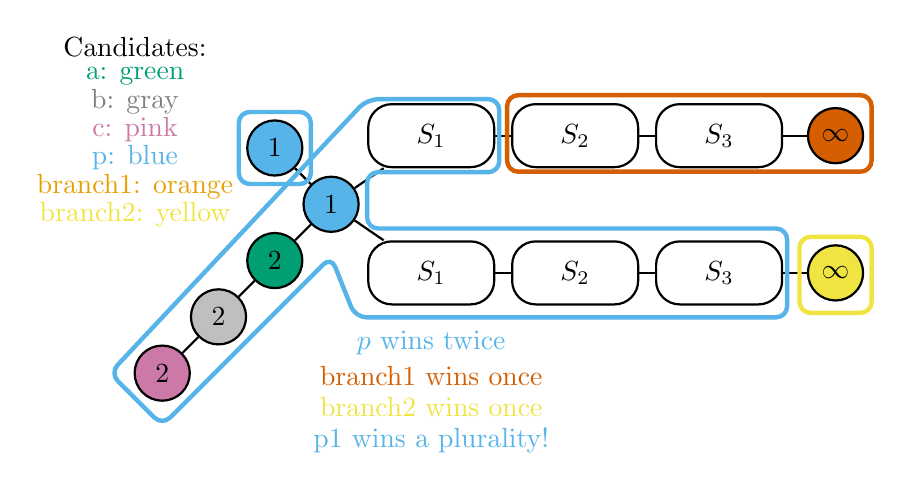
\begin{tikzpicture}
    \tikzstyle{node} = [circle, draw, thick, minimum size=0.7cm]
	\tikzstyle{edge} = [thick]
    \tikzstyle{gnode} = [rectangle, draw, thick, minimum width=1.6cm, minimum height=0.8cm, rounded corners=0.3cm]
    \tikzstyle{znode} = [circle, draw, minimum size=0.7cm, scale=0.83]

    \onslide<2-9> {
    \node (r) [node, fill=skyblue] {$1$};

    \node (e1) [node, fill=bluegreen, below left=0.2cm and 0.2cm of r] {$2$};
    \node (e2) [node, fill=lightgray, below left = 0.2cm and 0.2cm of e1] {$2$};
    \node (en) [node, fill=redpurple, below left=0.2cm and 0.2cm of e2] {$2$};

    \node (g11) [gnode, below right=0.2cm and 0.2cm of r] {$S_1$};
    \node (gi1) [gnode, right=0.2cm of g11] {$S_2$};
    \node (gn1) [gnode, right=0.2cm of gi1] {$S_3$};
    

    \node (g12) [gnode, above right=0.2cm and 0.2cm of r] {$S_1$};
    \node (gi2) [gnode, right=0.2cm of g12] {$S_2$};
    \node (gn2) [gnode, right=0.2cm of gi2] {$S_3$};

    \draw (r) edge [edge] (e1);
    \draw (e1) edge [edge] (e2);
    \draw (e2) edge [edge] (en);


    \draw (r) edge [edge] (g11);
    \draw (g11) edge [edge] (gi1);
    \draw (gi1) edge [edge] (gn1);
    

    \draw (r) edge [edge] (g12);
    \draw (g12) edge [edge] (gi2);
    \draw (gi2) edge [edge] (gn2);

        \node (candlabel) [text=black, above left= 1.5cm and 1.2cm of r] {Candidates:};
        \node (alabel) [text=bluegreen, below=-0.1cm of candlabel] {a: green};
        \node (blabel) [text=gray, below=-0.2cm of alabel] {b: gray};
        \node (clabel) [text=redpurple, below=-0.2cm of blabel] {c: pink};
        \node (plabel) [text=skyblue, below=-0.2cm of clabel] {p: blue};
    }

    \onslide<3-9> {
        \node (f1) [node, fill=yellow, right=0.3cm of gn1] {$\infty$};
        \node (f2) [node, fill=vermillion, right=0.3cm of gn2] {$\infty$};

        \draw (gn1) edge [edge] (f1);
        \draw (gn2) edge [edge] (f2);

        \node (b1label) [text=orange, below=-0.2cm of plabel] {branch1: orange};
        \node (b2label) [text=yellow, below=-0.2cm of b1label] {branch2: yellow};
    }

    \onslide<4-9> {
        \draw[ultra thick, rounded corners, color=yellow] ($(f1.north west) + (-0.2, 0.2)$) rectangle ($(f1.south east) + (0.2, -0.25)$);
        \draw[ultra thick, rounded corners, color=vermillion] ($(gi2.north west) + (-0.05, 0.1)$) rectangle ($(f2.south east) + (0.2, -0.2)$);
    }

    \onslide<5-9> {
        \node (u1) [node, fill=skyblue, above left=0.2cm and 0.2cm of r] {$1$};
        \draw (r) edge [edge] (u1);
    }

    \onslide<6-9> {
        \draw[ultra thick, rounded corners, color=skyblue] ($(u1.north west) + (-0.2, 0.2)$) rectangle ($(u1.south east) + (0.2, -0.2)$);
    }

    \onslide<7-9> {
        \draw[ultra thick, rounded corners, color=skyblue] ($(g12.north west) + (0, 0.05)$) -- ($(g12.north east) + (0.05, 0.05)$) -- ($(g12.south east) + (0.05, -0.05)$) -- ($(g12.south west) + (0, -0.05)$) -- ($(g11.north west) + (0, 0.15)$) -- ($(gn1.north east) + (0.05, 0.15)$) -- ($(gn1.south east) + (0.05, -0.15)$) -- ($(g11.south west) + (-0.15, -0.15)$) -- ($(r.south) + (0.0, -0.3)$) -- ($(en.south) + (0.0, -0.3)$) -- ($(en.west) + (-0.3, 0.0)$) -- cycle;
    }

    \onslide<8-9> {
        \node (pwins) [text=skyblue, below=0.2cm of g11] {$p$ wins twice};
        \node (b1wins) [text=vermillion, below=-0.1cm of pwins] {branch1 wins once};
        \node (b2wins) [text=yellow, below=-0.1cm of b1wins] {branch2 wins once};
        \node (pdub) [text=skyblue, below=-0.1cm of b2wins] {p1 wins a plurality!};
    }

    %\node (e1) [znode, fill=vermillion, below right=0.75cm and -0.56cm of g11] {$v_i^1$};
    %\node (e2) [minimum size = 0.5cm, right=0.25cm of e1] {$\dots$};
    %\node (en) [znode, fill=redpurple, right=0.25cm of e2] {$v_i^n$};
    %\node (x) [znode, fill=bluegreen, right=0.25cm of en] {$x_i$};
    %\node (y) [znode, fill=skyblue, right=0.25cm of x] {$y_i$};
    %\node (z) [znode, fill=orange, right=0.25cm of y] {$z_i$};

    %\draw (e1) edge [edge] (e2);
    %\draw (e2) edge [edge] (en);
    %\draw (en) edge [edge] (x);
    %\draw (x) edge [edge] (y);
    %\draw (y) edge [edge] (z);

    %\draw ($(gi1.south west) + (0.1, 0.1)$) -- ($(e1.north) + (-0.27, 0.15)$);
    %\draw ($(gi1.south east) + (-0.1, 0.1)$) -- ($(z.north) + (0.27, 0.15)$);
    %\draw[thick, rounded corners=0.3cm] ($(e1.north west) + (-0.25, 0.25)$) rectangle ($(z.south east) + (0.25, -0.25)$);
\end{tikzpicture}

		\end{center}
	\end{figure}
\end{frame}
	\begin{frame}
    \frametitle{Hardness Results}
    \begin{theorem}
        \gm is W[2]-Hard w.r.t. $k$ on trees with depth = 2.
    \end{theorem}
    
    \vspace{1.0cm}
    \onslide<2-3> {
    \begin{theorem}
        \gm is W[2]-Hard w.r.t. $k+\ell$ on trees with $\ell$ leaves.
    \end{theorem}
    }
    
    \vspace{1.0cm}
    \onslide<3> {
        Both of these results also apply when restricted to unit weights (vertices have weight 1).
    }
    
\end{frame}

\begin{frame}
    \frametitle{Unit Weight Results}
    \begin{itemize}
        \item Parameter: k
    \end{itemize}
	
\renewcommand{\arraystretch}{1.5}
\newcolumntype{Y}{>{\centering\arraybackslash}X}
\begin{tabularx}{\textwidth}{|c||c|Y|Y|Y|}
	\hline

	&
	Planar &
	Trees &
	Paths &
	Stars \\

	\hline
	\hline

	XP &
	\cellcolor{gray} Ito 3.1 &
	\cellcolor{blue} Ito 4.1 &
	\cellcolor{blue} &
	\cellcolor{blue} \\

	\hline

	FPT &
	\cellcolor{gray} &
	\cellcolor{red} Fraser 3 &
	\cellcolor{blue} Gupta 1.2 &
	\cellcolor{blue} \\

	\hline

	Poly &
	\cellcolor{gray} &
	\cellcolor{gray} Ito 3.3 &
	\cellcolor{gray} Bentert 1 &
	\cellcolor{blue} Ito 4.2 \\

	\hline
\end{tabularx}
\renewcommand{\arraystretch}{1}

    \begin{itemize}
        \item Parameter: k, with unit weights
    \end{itemize}
    
\renewcommand{\arraystretch}{1.5}
\setlength{\tabcolsep}{5pt}
\onslide<2>{\setlength{\tabcolsep}{5pt}}
\begin{tabular}{|c||c|c|c|c|}
	\hline

	&
	Planar &
	Trees &
	Paths &
	Stars \\

	\hline
	\hline

	XP &
	\cellcolor{white} &
	\cellcolor{skyblue} Ito &
	\cellcolor{skyblue} &
	\cellcolor{skyblue} \\

	\hline

	FPT &
	\only<2>{\cellcolor{gray}} &
    \only<2>{\cellcolor{gray}}\only<2>{Fraser} \only<1>{\textcolor{white}{Fraser}} &
	\cellcolor{skyblue} Gupta &
	\cellcolor{skyblue} \\

	\hline

	Poly &
	\cellcolor{lightgray} &
	\cellcolor{lightgray} Ito &
	\cellcolor{lightgray} Bentert &
	\cellcolor{skyblue} Ito \\

	\hline
\end{tabular}
\renewcommand{\arraystretch}{1}
\end{frame}

\begin{frame}
    \frametitle{FPT Results}
    \begin{theorem}
        \gm is FPT on trees with a constant number of leaves
    \end{theorem}
    
    \vspace{1.0cm}
    \onslide<2> {
        Algorithm strategy:
        \begin{itemize}
            \item Use brute force to predetermine all possible districts on a branch
            \item Repeat this until we have a set of disjoint paths
            \item Gupta et al. can solve a set of disjoint paths
        \end{itemize}
    }
\end{frame}


\begin{frame}
    \frametitle{FPT Algorithm}

    \begin{figure}
		\begin{center}
			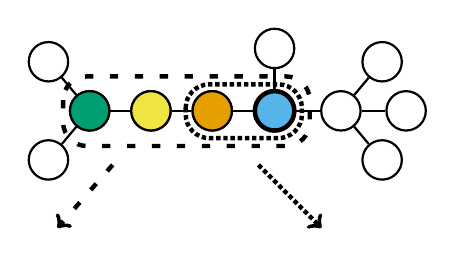
\begin{tikzpicture}
    \tikzstyle{node} = [circle, draw, thick, minimum size=0.5cm]
	\tikzstyle{edge} = [thick]

    \onslide<1> {
        \node (r) [node, red, fill=skyblue, ultra thick] {};
    }
    \node (l) [node, fill=white, above=0.25cm of r] {};

    \onslide<1> {
        \node (p1) [node, fill=white, left=0.25cm of r] {};
        \node (p2) [node, fill=white, left=0.25cm of p1] {};
        \node (b1) [node, fill=white, left=0.25cm of p2] {};
        \draw (r) edge [edge] (p1);
    }
    
    \node (b11) [node, fill=white, above left=0.25cm and 0.15cm of b1] {};
    \node (b12) [node, fill=white, below left=0.25cm and 0.15cm of b1] {};

    \node (b2) [node, fill=white, right=0.3cm of r] {};
    \node (b21) [node, fill=white, above right=0.25cm and 0.15cm of b2] {};
    \node (b22) [node, fill=white, right=0.3cm of b2] {};
    \node (b23) [node, fill=white, below right=0.25cm and 0.15cm of b2] {};

    \draw (r) edge [edge] (l);
    \onslide<1> {
        \draw (r) edge [edge, red] (p1);
    }
    
    \draw (r) edge [edge] (b2);

    \draw (p1) edge [edge] (p2);
    \draw (p2) edge [edge] (b1);
    \draw (b1) edge [edge] (b11);
    \draw (b1) edge [edge] (b12);

    \draw (b2) edge [edge] (b21);
    \draw (b2) edge [edge] (b22);
    \draw (b2) edge [edge] (b23);

    \onslide<2-4> {
        \node (r) [node, fill=skyblue, ultra thick] {};
        \node (p1) [node, fill=orange, left=0.25cm of r] {};
        \node (p2) [node, fill=yellow, left=0.25cm of p1] {};
        \node (b1) [node, fill=bluegreen, left=0.25cm of p2] {};
        \draw (r) edge [edge] (p1);
    }

    \onslide<4> {
        \draw[ultra thick, rounded corners=3mm, densely dotted, color=black] ($(p1.north west) + (-0.15, 0.15)$) rectangle ($(r.south east) + (0.15, -0.15)$);
    }
    \onslide<3-4> {
        \draw[ultra thick, rounded corners=3mm, loosely dashed, color=black] ($(b1.north west) + (-0.15, 0.25)$) rectangle ($(r.south east) + (0.25, -0.25)$);

    \draw[->, ultra thick, color=black, loosely dashed] ($(p2.south west) + (-0.3, -0.5)$) -> ($(p2.south west) + (-1, -1.3)$);
    }
    
    \onslide<4> {
        \draw[->, ultra thick, color=black, densely dotted] ($(p1.south east) + (0.4, -0.5)$) -> ($(p1.south east) + (1.2, -1.3)$);
    }
\end{tikzpicture}

		\end{center}
	\end{figure}

    \begin{figure}
        \begin{center}
            \onslide<3-4> {
                \begin{tikzpicture}
    \tikzstyle{node} = [circle, draw, thick, minimum size=0.5cm]
	\tikzstyle{edge} = [thick]

    \node (b1) [node, ultra thick]  {};

    \node (l) [node, fill=white, above=0.25cm of r] {};

    \node (b11) [node, fill=white, above left=0.1cm and 0.3cm of b1] {};
    \node (b12) [node, fill=white, below left=0.1cm and 0.3cm of b1] {};

    \node (b2) [node, fill=white, right=0.3cm of b1] {};
    \node (b21) [node, fill=white, above right=0.25cm and 0.15cm of b2] {};
    \node (b22) [node, fill=white, right=0.3cm of b2] {};
    \node (b23) [node, fill=white, below right=0.25cm and 0.15cm of b2] {};

    \draw (b1) edge [edge] (b11);
    \draw (b1) edge [edge] (b12);
    \draw (b1) edge [edge] (l);
    \draw (b1) edge [edge] (b2);

    \draw (b2) edge [edge] (b21);
    \draw (b2) edge [edge] (b22);
    \draw (b2) edge [edge] (b23);

    \clip ($(b1)$)circle (0.2275cm);
    \begin{scope}
        \rotatebox{-45}{
            \fill[orange] ($(b1.north)$) rectangle ($(b1.west)$);
            \fill[skyblue] ($(b1.north)$) rectangle ($(b1.east)$);
            \fill[bluegreen] ($(b1.south)$) rectangle ($(b1.west)$);
            \fill[yellow] ($(b1.south)$) rectangle ($(b1.east)$);
        }
    \end{scope}
\end{tikzpicture}

            }
            \hspace{2.0cm}
            \onslide<4> {
                \begin{tikzpicture}
    \tikzstyle{node} = [circle, draw, thick, minimum size=0.5cm]
	\tikzstyle{edge} = [thick]

    \node (p1) [node, ultra thick] {};
    \node (l) [node, fill=white, above=0.25cm of r] {};

    \node (p2) [node, fill=yellow, left=0.25cm of p1] {};
    \node (b1) [node, fill=bluegreen, left=0.25cm of p2]  {};
    \node (b11) [node, fill=white, above left=0.25cm and 0.15cm of b1] {};
    \node (b12) [node, fill=white, below left=0.25cm and 0.15cm of b1] {};

    \node (b2) [node, fill=white, right=0.3cm of p1] {};
    \node (b21) [node, fill=white, above right=0.25cm and 0.15cm of b2] {};
    \node (b22) [node, fill=white, right=0.3cm of b2] {};
    \node (b23) [node, fill=white, below right=0.25cm and 0.15cm of b2] {};

    \draw (p1) edge [edge] (l);
    \draw (p2) edge [edge] (b1);
    \draw (b1) edge [edge] (b11);
    \draw (b1) edge [edge] (b12);

    \draw (p1) edge [edge] (b2);
    \draw (b2) edge [edge] (b21);
    \draw (b2) edge [edge] (b22);
    \draw (b2) edge [edge] (b23);

    \clip ($(p1)$)circle (0.2275cm);
    \begin{scope}
        \fill[orange] ($(p1.south)$) rectangle ($(p1.north) + (-0.25, 0)$);
        \fill[skyblue] ($(p1.south)$) rectangle ($(p1.north) + (0.25, 0)$);
    \end{scope}


\end{tikzpicture}

            }
        \end{center}
    \end{figure}
\end{frame}
	\begin{frame}[t]
    \frametitle{Results Overview}
    \begin{itemize}
        \item \gm is W[2]-Hard parameterized by $k$ on trees with depth=2, even with unit weights
        \item \gm is W[2]-Hard parameterized by $k+\ell$ on trees with $\ell$ leaves, even with unit weights
        \item \gm is FPT by $k$ on trees with a constant number of leaves
    \end{itemize}
    \vspace{1.0cm}
\end{frame}

\begin{frame}[t]
    \frametitle{Thank you!}
    Any questions?
\end{frame}

\end{document}